\documentclass[a4paper]{article}
\usepackage{graphicx,tikz} 
\usepackage{multirow}
\usepackage{enumitem}
\usepackage{amssymb}
\usepackage{amsmath}
\usepackage{amsthm}
\usepackage{xcolor}
\usepackage{multicol}
\usepackage{multirow}
\usepackage{array}
\usepackage{animate}
\usepackage{amsthm}
\usepackage{caption}
\usepackage{minted}
\usepackage{forest}
\usepackage{fancyhdr}
\usepackage{geometry}
	\geometry{
		total = {160mm, 237mm},
		left = 30mm,
		right = 35mm,
		top = 35mm,
        bottom = 30mm,
        headheight=2cm
	}
\renewcommand{\headrulewidth}{0pt}

\graphicspath{{C:/Users/teoso/OneDrive/Documents/Tugas Kuliah/Template Math Depart/}}

\newcommand{\R}{\mathbb{R}}
\newcommand{\N}{\mathbb{N}}
\newcommand{\Z}{\mathbb{Z}}
\newcommand{\Q}{\mathbb{Q}}
\newcommand{\jawab}{\textbf{Solusi}:}

\definecolor{bg}{rgb}{0.95, 0.95, 0.92}

\setminted[cpp]{bgcolor=bg,frame=single,bgcolorpadding=1mm,escapeinside=||}

\title{Soal OSK Informatika}
\author{Graf dan Pohon}
\date{26 April 2025}

\begin{document}
\maketitle
\begin{enumerate}
  \item\textbf{(OSK 2022)} Diketahui ada enam kota A, B, C, D, E, dan F sebagai berikut:

  \begin{center}
  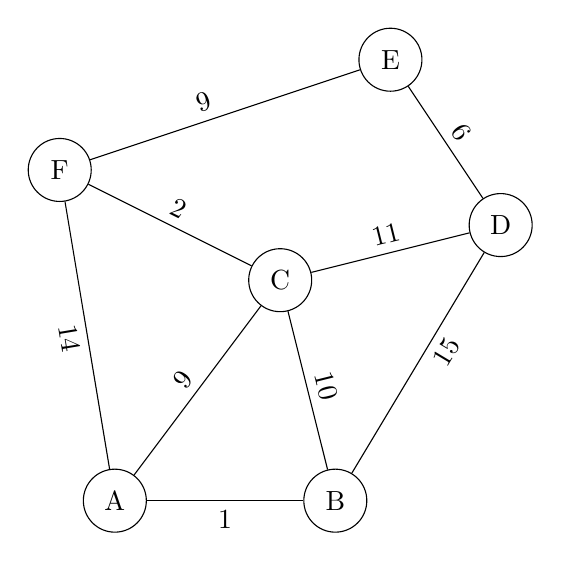
\begin{tikzpicture}[scale=1.4]
  
    \node[circle, draw, minimum size=0.8cm] (A) at (0,0) {A};
    \node[circle, draw, minimum size=0.8cm] (B) at (2,0) {B};
    \node[circle, draw, minimum size=0.8cm] (C) at (1.5,2) {C};
    \node[circle, draw, minimum size=0.8cm] (D) at (3.5,2.5) {D};
    \node[circle, draw, minimum size=0.8cm] (E) at (2.5,4) {E};
    \node[circle, draw, minimum size=0.8cm] (F) at (-0.5,3) {F};
  
    \draw (A) -- node[below,sloped] {1} (B);
    \draw (A) -- node[above,sloped] {9} (C);
    \draw (A) -- node[below,sloped] {14} (F);
    \draw (B) -- node[above,sloped] {10} (C);
    \draw (B) -- node[below right,sloped] {15} (D);
    \draw (C) -- node[above,sloped] {2} (F);
    \draw (C) -- node[above,sloped] {11} (D);
    \draw (D) -- node[above,sloped] {6} (E);
    \draw (E) -- node[above left,sloped] {9} (F);
  
  \end{tikzpicture}
  \end{center}
  
  Dua kota dikatakan terhubung jika ada jalan (divisualisasikan sebagai garis) yang menghubungkan keduanya dengan jarak dalam kilometer. Pak Dengklek ditugasi untuk memasang kabel internet di atas beberapa jalan yang ada sedemikian sehingga setiap kota bisa terhubung baik secara langsung maupun tidak langsung (melalui kota lainnya). Berapa panjang kabel minimal yang harus disiapkan oleh Pak Dengklek?
  \begin{multicols}{5}
    \begin{itemize}
      \item[A.] 25
      \item[B.] 27
      \item[C.] 29
      \item[D.] 32
      \item[E.] 33
    \end{itemize} 
  \end{multicols}


  \item\textbf{(OSK 2022)} Diketahui 8 buah kota dengan label 0, 1, 2, ..., 7 yang masing-masing terhubung dengan sebuah jalan. Setiap jalan bersifat satu arah.

  \begin{center}
  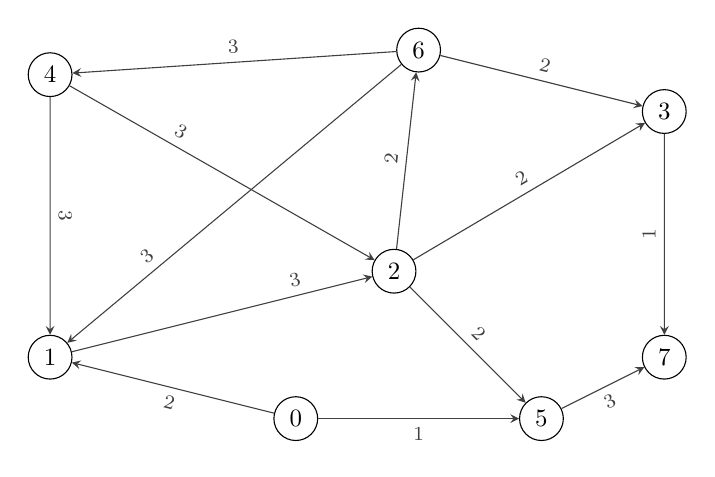
\begin{tikzpicture}[->, >=stealth, auto, node distance=1cm, scale=1.2, every node/.style={scale=0.9},scale=1.3]
    % Nodes
    \node[circle, draw] (0) at (0,0) {0};
    \node[circle, draw] (1) at (-2,0.5) {1};
    \node[circle, draw] (2) at (0.8,1.2) {2};
    \node[circle, draw] (3) at (3,2.5) {3};
    \node[circle, draw] (4) at (-2,2.8) {4};
    \node[circle, draw] (5) at (2,0) {5};
    \node[circle, draw] (6) at (1,3) {6};
    \node[circle, draw] (7) at (3,0.5) {7};
  
    % Edges
    
    \draw[darkgray] (4) -- (1) node[midway, above,sloped] {\footnotesize 3};
    \draw[darkgray] (2) -- (6) node[midway, above,sloped] {\footnotesize 2};
    
    \draw[darkgray] (1) -- (2) node[midway, above left,sloped,pos=0.8] {\footnotesize 3};
    \draw[darkgray] (2) -- (5) node[midway, above,sloped] {\footnotesize 2};
    \draw[darkgray] (6) -- (1) node[midway,sloped, above left,pos=0.7] {\footnotesize 3};
    \draw[darkgray] (4) -- (2) node[midway,sloped, above right,pos=0.3] {\footnotesize 3};

    \draw[darkgray] (0) -- (1) node[midway,sloped, below] {\footnotesize 2};
    \draw[darkgray] (2) -- (3) node[midway,sloped, above] {\footnotesize 2};
    \draw[darkgray] (3) -- (7) node[midway,sloped, above] {\footnotesize 1};
    \draw[darkgray] (0) -- (5) node[midway,sloped, below] {\footnotesize 1};
    \draw[darkgray] (6) -- (4) node[midway,sloped, above] {\footnotesize 3};
    \draw[darkgray] (6) -- (3) node[midway,sloped, above] {\footnotesize 2};
    \draw[darkgray] (5) -- (7) node[midway,sloped, below] {\footnotesize 3};
  
  \end{tikzpicture}
  \end{center}
  
  Diketahui pula waktu tempuh dari satu kota ke kota yang lain melalui masing-masing jalan sesuai dengan nilai yang ditunjukkan pada masing-masing jalan penghubung (dalam satuan jam). Waktu tempuh antara dua buah kota didefinisikan sebagai nilai terkecil dari total waktu tempuh jalan-jalan yang harus dilewati untuk berpindah dari satu kota ke kota lainnya. 
  
  Misalnya, waktu tempuh dari kota 2 ke 7 adalah 3, karena kita dapat melalui jalur 2 → 3 (waktu tempuh = 2) dan jalur 3 → 7 (waktu tempuh = 1), sehingga total = 2 + 1 = 3. Kota manakah yang waktu tempuhnya dari kota 0 paling besar?
  \begin{multicols}{5}
    \begin{itemize}
      \item[A.] 3
      \item[B.] 4
      \item[C.] 5
      \item[D.] 6
      \item[E.] 7
  \end{itemize}
  \end{multicols}

  \item\textbf{(OSK 2023)} Bebek-bebek Pak Dengklek tinggal pada salah satu dari tujuh buah kandang yang dinomori 0 sampai 6. Terdapat beberapa jalan setapak yang menghubungi sepasang kandang. Untuk pergi dari satu kandang ke kandang lainnya, Pak Dengklek harus menelusuri jalan setapak tersebut. Berikut adalah peta kandang-kandang dan jalan setapak yang menghubungkan mereka:

  \begin{center}
  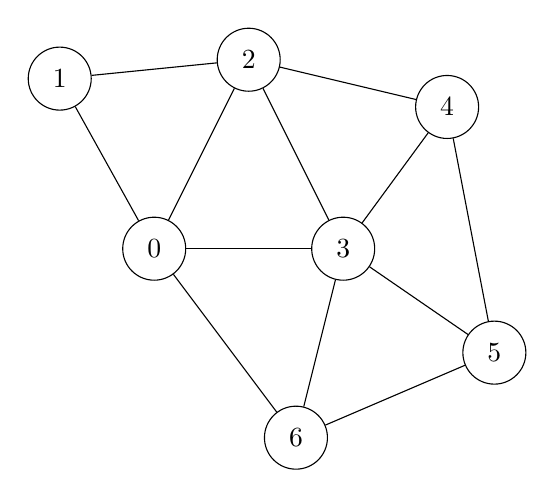
\begin{tikzpicture}[scale=1.2, every node/.style={circle, draw, minimum size=0.8cm}]
    \node (0) at (-1,0) {0};
    \node (1) at (-2,1.8) {1};
    \node (2) at (0,2) {2};
    \node (3) at (1,0) {3};
    \node (4) at (2.1,1.5) {4};
    \node (5) at (2.6,-1.1) {5};
    \node (6) at (0.5,-2) {6};
  
    \draw (0) -- (1);
    \draw (0) -- (2);
    \draw (0) -- (3);
    \draw (0) -- (6);
    \draw (1) -- (2);
    \draw (2) -- (3);
    \draw (2) -- (4);
    \draw (3) -- (4);
    \draw (3) -- (5);
    \draw (3) -- (6);
    \draw (4) -- (5);
    \draw (5) -- (6);
  \end{tikzpicture}
  \end{center}
  
  Pak Dengklek sekarang berada di kandang bernomor 0, dan ia ingin menyiram tanaman yang berada di tiap jalan setapak. Maka, Pak Dengklek ingin menelusuri semua jalan setapak setidaknya sekali. Pak Dengklek dapat menelusuri sebuah jalan setapak dalam satu menit. Berapa waktu minimum (dalam menit) yang dibutuhkan Pak Dengklek untuk menelusuri semua jalan setapak setidaknya sekali?
  \begin{multicols}{5}
    \begin{itemize}
      \item[A.] 12
      \item[B.] 13
      \item[C.] 14
      \item[D.] 15
      \item[E.] 16
    \end{itemize}
  \end{multicols}

  \item\textbf{(OSK 2023)} Pemerintah Kabupaten Algoria berniat untuk menghubungkan keenam kecamatannya dengan jaringan Internet super cepat untuk meningkatkan perekonomian rakyatnya. Jaringan tersebut akan dibangun dengan membuat kabel yang menghubungkan antar kecamatan, sedemikian rupa sehingga antar setiap pasang kecamatan harus ada jalur melalui kabel-kabel yang menghubungkan keduanya (baik secara langsung maupun melalui kecamatan-kecamatan lain).

  Lebih lanjut, setiap kabel yang menghubungkan dua buah kecamatan harus dibangun melalui jalan yang menghubungkan dua buah kecamatan tersebut. Terdapat 9 jalan yang menghubungkan 6 kecamatan tersebut, sebagaimana terlihat pada gambar di bawah ini.
  
  \begin{center}
  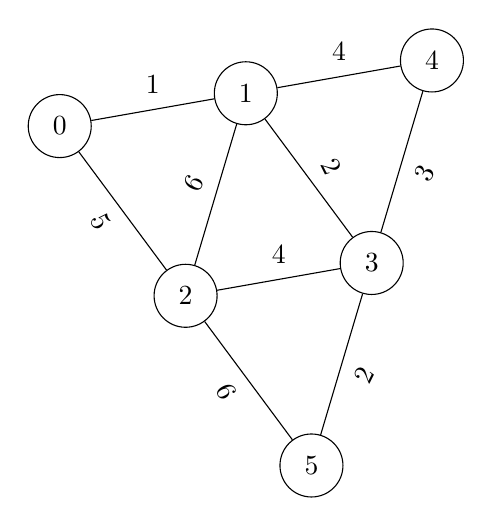
\begin{tikzpicture}[every node/.style={circle, draw, minimum size=0.8cm}, scale=1.2,rotate=10]
    \node (0) at (0,0) {0};
    \node (1) at (2,0) {1};
    \node (2) at (1,-2) {2};
    \node (3) at (3,-2) {3};
    \node (4) at (4,0) {4};
    \node (5) at (2,-4) {5};
  
    \draw (0) -- node[minimum size=0cm,draw=none,above,sloped] {1} (1);
    \draw (0) -- node[minimum size=0cm,draw=none,below,sloped] {5} (2);
    \draw (1) -- node[minimum size=0cm,draw=none,above,sloped] {6} (2);
    \draw (1) -- node[minimum size=0cm,draw=none,above,sloped] {4} (4);
    \draw (2) -- node[minimum size=0cm,draw=none,above,sloped] {4} (3);
    \draw (2) -- node[minimum size=0cm,draw=none,below,sloped] {6} (5);
    \draw (3) -- node[minimum size=0cm,draw=none,above,sloped] {2} (1);
    \draw (3) -- node[minimum size=0cm,draw=none,below,sloped] {3} (4);
    \draw (3) -- node[minimum size=0cm,draw=none,below,sloped] {2} (5);

  \end{tikzpicture}
  \end{center}
  
  Pak Dengklek yang ditugaskan untuk merencanakan pembangunan jaringan Internet tersebut, telah menghitung bahwa biaya terkecil untuk menghubungkan semua kecamatan adalah 12, sebagaimana ditunjukkan pada gambar di bawah ini.
  
  \begin{center}
    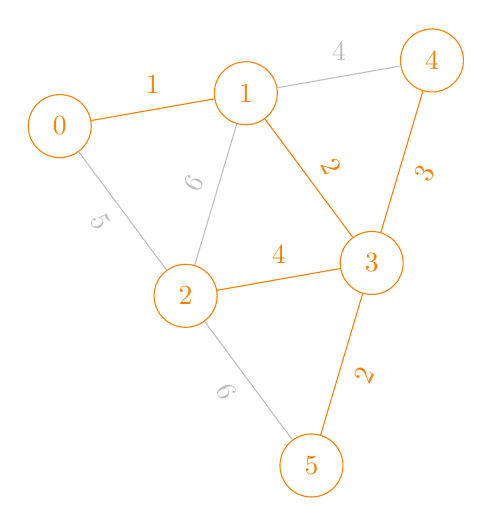
\begin{tikzpicture}[every node/.style={circle, draw, minimum size=0.8cm}, scale=1.2,rotate=10]
      \node[orange] (0) at (0,0) {0};
      \node[orange] (1) at (2,0) {1};
      \node[orange] (2) at (1,-2) {2};
      \node[orange] (3) at (3,-2) {3};
      \node[orange] (4) at (4,0) {4};
      \node[orange] (5) at (2,-4) {5};
    
      \draw[orange] (0) -- node[minimum size=0cm,draw=none,above,sloped] {1} (1);
      \draw[lightgray] (0) -- node[minimum size=0cm,draw=none,below,sloped] {5} (2);
      \draw[lightgray] (1) -- node[minimum size=0cm,draw=none,above,sloped] {6} (2);
      \draw[lightgray] (1) -- node[minimum size=0cm,draw=none,above,sloped] {4} (4);
      \draw[orange] (2) -- node[minimum size=0cm,draw=none,above,sloped] {4} (3);
      \draw[lightgray] (2) -- node[minimum size=0cm,draw=none,below,sloped] {6} (5);
      \draw[orange] (3) -- node[minimum size=0cm,draw=none,above,sloped] {2} (1);
      \draw[orange] (3) -- node[minimum size=0cm,draw=none,below,sloped] {3} (4);
      \draw[orange] (3) -- node[minimum size=0cm,draw=none,below,sloped] {2} (5);
  
    \end{tikzpicture}
  \end{center}
  
  Namun, ketika Pak Dengklek ingin mengusulkan rencana pembangunan jalan sebagaimana terlihat pada gambar di atas, oleh atasannya rencana tersebut ditolak. Lebih lanjut, sang atasan meminta Pak Dengklek mencari berapakah biaya terkecil kedua setelah nilai biaya terkecil (12) yang diusulkan Pak Dengklek tadi?
  
  \textbf{Jawaban:} \underline{\hspace{2cm}} \quad \emph{(tuliskan jawaban dalam bentuk ANGKA saja)}

  \item\textbf{(OSK 2023)} Pak Dengklek memiliki 13 buah benda pusaka yang dilabeli A, B, C, D, E, F, G, H, I, J, K, L, dan M dalam sebuah tanah yang masing-masing memiliki hubungan sebagai berikut: 
  \begin{center}
    \begin{forest}
    for tree={
        draw,
        circle,
        minimum size=1.2em,
        inner sep=2pt,
        l sep=20pt,
        s sep=10pt,
        anchor=center,
        grow'=south,
        child anchor=north
    }
    [A
      [D
        [M]
        [L]
        [K]
      ]
      [C
        [J]
        [I]
        [H]
      ]
      [B
        [G]
        [F]
        [E]
      ]
    ]
    \end{forest}
    \end{center}
    Dari gambar di atas diketahui bahwa benda pusaka B, C, dan D memiliki kekuatan yang diturunkan dari benda pusaka A, benda pusaka E, F, dan G memiliki kekuatan yang diturunkan dari benda pusaka B, dst. Kemudian Pak Dengklek mendefinisikan sebuah fungsi \texttt{kiri(X)}, \texttt{tengah(X)} dan \texttt{kanan(X)} suatu benda pusaka X yang didefinisikan sebagai benda pusaka yang posisinya sebagai turunan benda pusaka X sebelah kiri, tengah, dan kanan. Sebagai contoh \texttt{kiri(B)=E}, \texttt{tengah(B)=F}, \texttt{kanan(B)=G}, tentunya benda pusaka yang tidak memiliki turunan, nilai fungsi kiri, tengah, dan kananya akan bernilai kosong. Selanjutnya Pak Dengklek mendefinisikan sebuah cara untuk mencari benda pusaka yang dia miliki yaitu dengan cara membuat fungsi cari sebagai berikut: 
    \begin{minted}{cpp}
  fungsi cari(x):
    //jika nilai x tidak kosong:
    cari(kiri(x));
    cari(tengah(x));
    cari(kanan(x));
    //letakkan x dalam box
    \end{minted}
    Setiap kali menemukan benda pusaka, Pak Dengklek akan meletakkannya dalam sebuah boks kosong pada posisi paling atas. Jika Pak Dengklek memulai pencarian dengan benda pusaka A yaitu cari(A) sampai semua benda pusaka ditemukan, tuliskan urutan benda pusaka dalam boks mulai dari posisi paling atas sampai posisi paling bawah. 

    \textbf{Jawaban:} \underline{\hspace{1cm}} \quad \textit{(tuliskan jawaban dalam bentuk HURUF KAPITAL saja tanpa spasi)}

    \item\textbf{(OSK 2024)} Pak Dengklek mengajari bebek-bebeknya untuk menggambar denah desa masa kecilnya. Pak Dengklek mengatakan bahwa di desa tersebut hanya terdapat 6 buah rumah yang dihubungkan oleh 8 ruas jalan sebagai berikut:

    \begin{itemize}
        \item Rumah 1 terhubung ruas jalan dengan rumah 2, 3, dan 4.
        \item Rumah 2 terhubung ruas jalan dengan rumah 1, 3, dan 5.
        \item Rumah 3 terhubung ruas jalan dengan rumah 1, 2, dan 6.
        \item Rumah 4 terhubung ruas jalan dengan rumah 1 dan 6.
        \item Rumah 5 terhubung ruas jalan dengan rumah 2 dan 6.
        \item Rumah 6 terhubung ruas jalan dengan rumah 3, 4, dan 5.
    \end{itemize}
    
    Bebek-bebek Pak Dengklek menggambar denahnya dengan lingkaran yang menunjukkan rumah dan garis yang menunjukkan ruas jalan. Namun karena mereka usil, mereka tidak menuliskan nomor rumah masing-masing.
    \begin{center}
      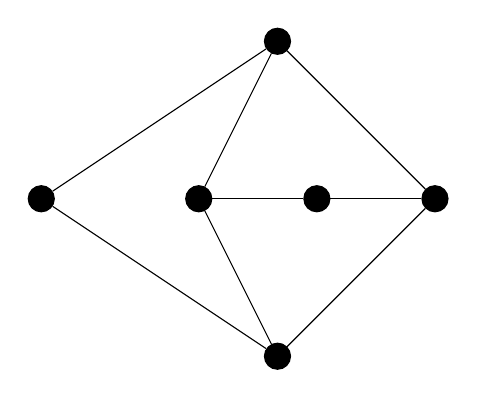
\begin{tikzpicture}[scale=2, every node/.style={circle, draw, fill=black}]
          % Nodes
          \node (A) at (0,1) {};
          \node (B) at (-1.5,0) {};
          \node (C) at (-0.5,0) {};
          \node (D) at (1,0) {};
          \node (E) at (0,-1) {};
          \node (F) at (0.25,0) {};
          
          % Edges
          \draw (A) -- (B);
          \draw (A) -- (C);
          \draw (A) -- (D);
          \draw (B) -- (E);
          \draw (C) -- (E);
          \draw (D) -- (E);
          \draw (C) -- (F);
          \draw (D) -- (F);
      \end{tikzpicture}
    \end{center}
    \textbf{\underline{BENAR atau SALAH}}: Jika nomor-nomor rumahnya dilabeli secara tepat, maka denah tersebut bisa jadi sudah sesuai dengan denah yang diinginkan oleh Pak Dengklek.
    
    \textbf{Tuliskan jawaban dalam bentuk BENAR/SALAH dengan huruf kapital.}
    
    
\end{enumerate}
\end{document}